\section{User Study}

We conducted a user study in order to evaluate the accuracy whether our hypothesis was true or not.

......

\subsection{Method}

We divided users into two groups by whether they have the same native language or not. So there are native language and foreign language group respectively. Foreign language group are required to use their native language to communicate with each other. About our experiment, every team will have two players and be placed in two different room. Players play Mote Robot with each other through Internet connection. Totally we tested 24 groups with 48 users, inclusive of 12 native language groups and 12 foreign language groups.

In our experiment, we provided three different types of communication manners to play Mute Robot:
\begin{enumerate}
    \item Speaking: 
    Traditional gameplay manner, user can communicate through speaking language.
    \item Body Language: 
    players can communicate through body language.
    \item using Speaking and Body Language together: 
    players can communicate with each other through speaking language and body language.
\end{enumerate}

In order to eliminate order effects, each user played Mute Robot with counterbalance by administering the various types of game in different sequence. After playing each type of Mute Robot, players will fill out an eSFQ\cite{} questionnaire to evaluate gameplay experience. Besides, When players finished all three types of Mute Robot, they will need to fill out another overall questionnaire and proceed user interview. It needs about 1 hour to finish our user study experiment. We would conduct video recording at all experiment process and used these video to do CPMs\cite{} (see Figure~\ref{fig:US1}). , which used to evaluate user gameplay experience.

\begin{figure}[!h]
\centering
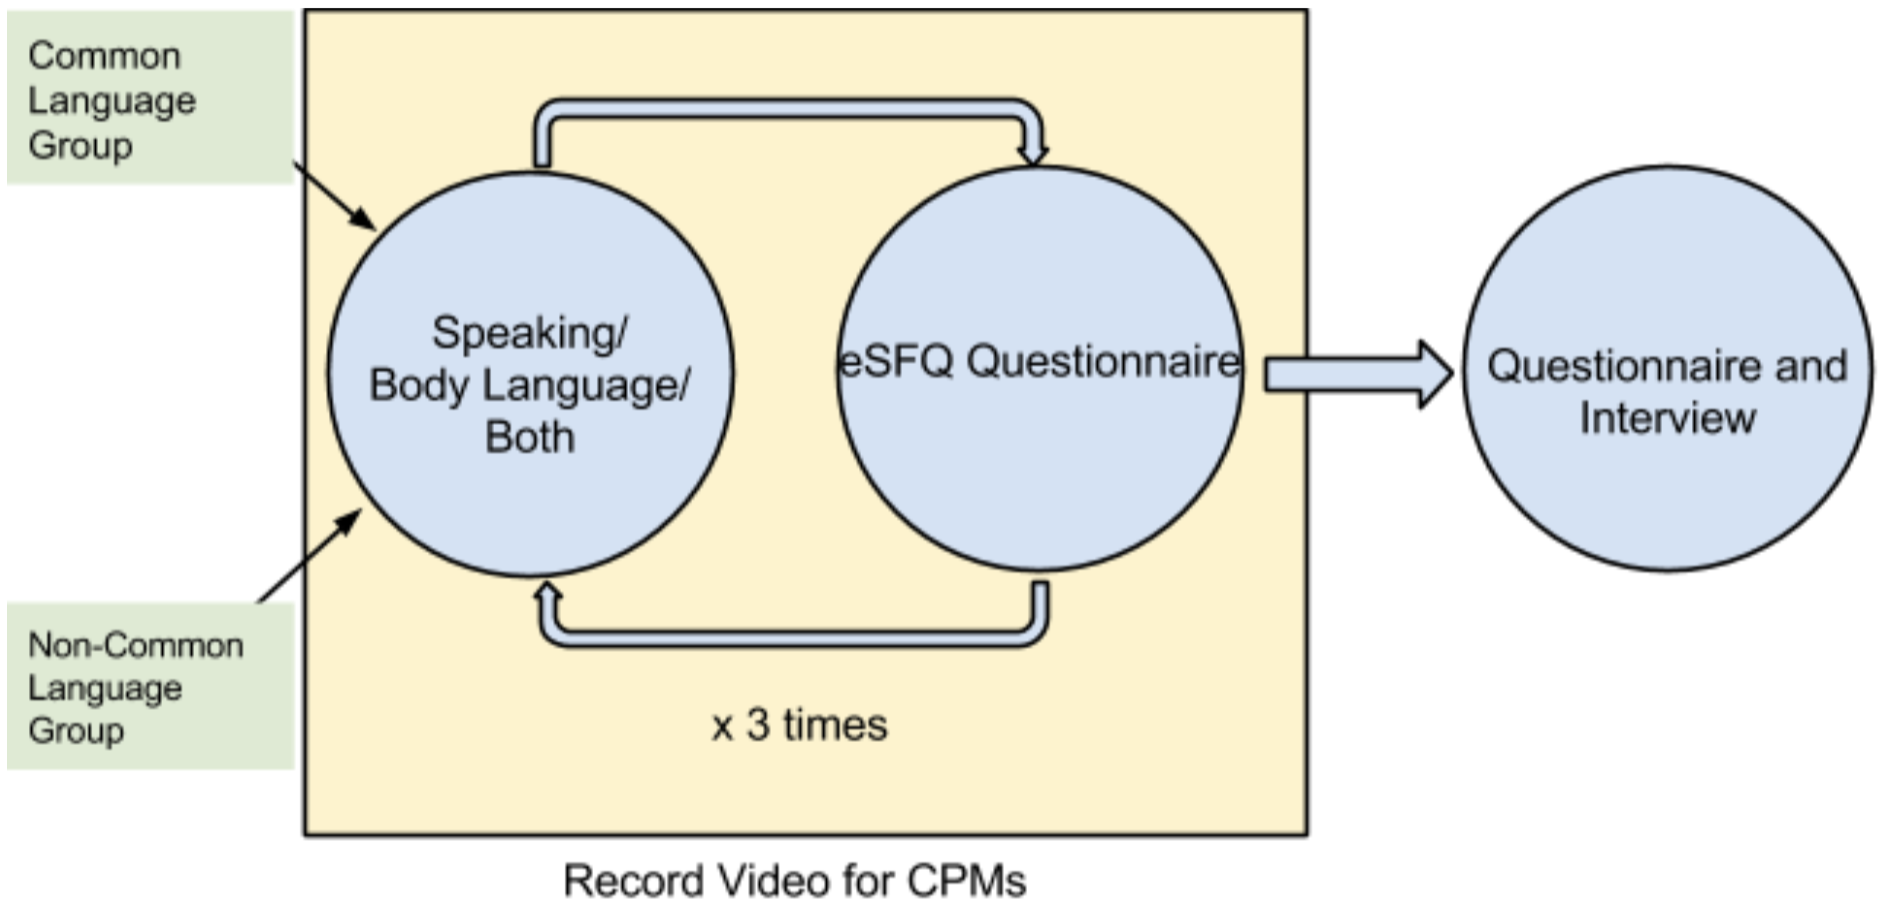
\includegraphics[width=0.9\columnwidth]{Figures/US_F1.png}
\caption{?????????}
\label{fig:US1}
\end{figure}



\subsubsection{Process}

\subsection{Observation}

\subsubsection{Communication Pattern}

\subsection{Result}

\subsection{Discussion}